%%% template.tex
%%%
%%% This LaTeX source document can be used as the basis for your technical
%%% paper or abstract. Intentionally stripped of annotation, the parameters
%%% and commands should be adjusted for your particular paper - title, 
%%% author, article DOI, etc.
%%% The accompanying ``template.annotated.tex'' provides copious annotation
%%% for the commands and parameters found in the source document. (The code
%%% is identical in ``template.tex'' and ``template.annotated.tex.'')

\documentclass[conference]{acmsiggraph}

\TOGonlineid{45678}
\TOGvolume{0}
\TOGnumber{0}
\TOGarticleDOI{1111111.2222222}
\TOGprojectURL{}
\TOGvideoURL{}
\TOGdataURL{}
\TOGcodeURL{}

\title{3D Printing for Mobile Robots}

\author{Andrew Spielberg\thanks{e-mail:aespielberg@csail.mit.edu} \and Vicki Crosson\thanks{e-mail:viccro.mit@gmail.com}}
\pdfauthor{Andrew Spielberg and Vicki Crosson}

\keywords{3D Printing, Robotics, 3Doodler, Trajectory Controller}

\usepackage{amsthm}
\usepackage{algorithm}
\usepackage[noend]{algpseudocode}
\usepackage{caption}
\usepackage{subcaption}
%\usepackage[subfigure]{ccaption}

\makeatletter
\def\BState{\State\hskip-\ALG@thistlm}
\makeatother

\newtheorem{theorem}{Theorem}[section]
\newtheorem{lemma}[theorem]{Lemma}
\newtheorem{proposition}[theorem]{Proposition}
\newtheorem{corollary}[theorem]{Corollary}



\begin{document}

%% \teaser{
%%   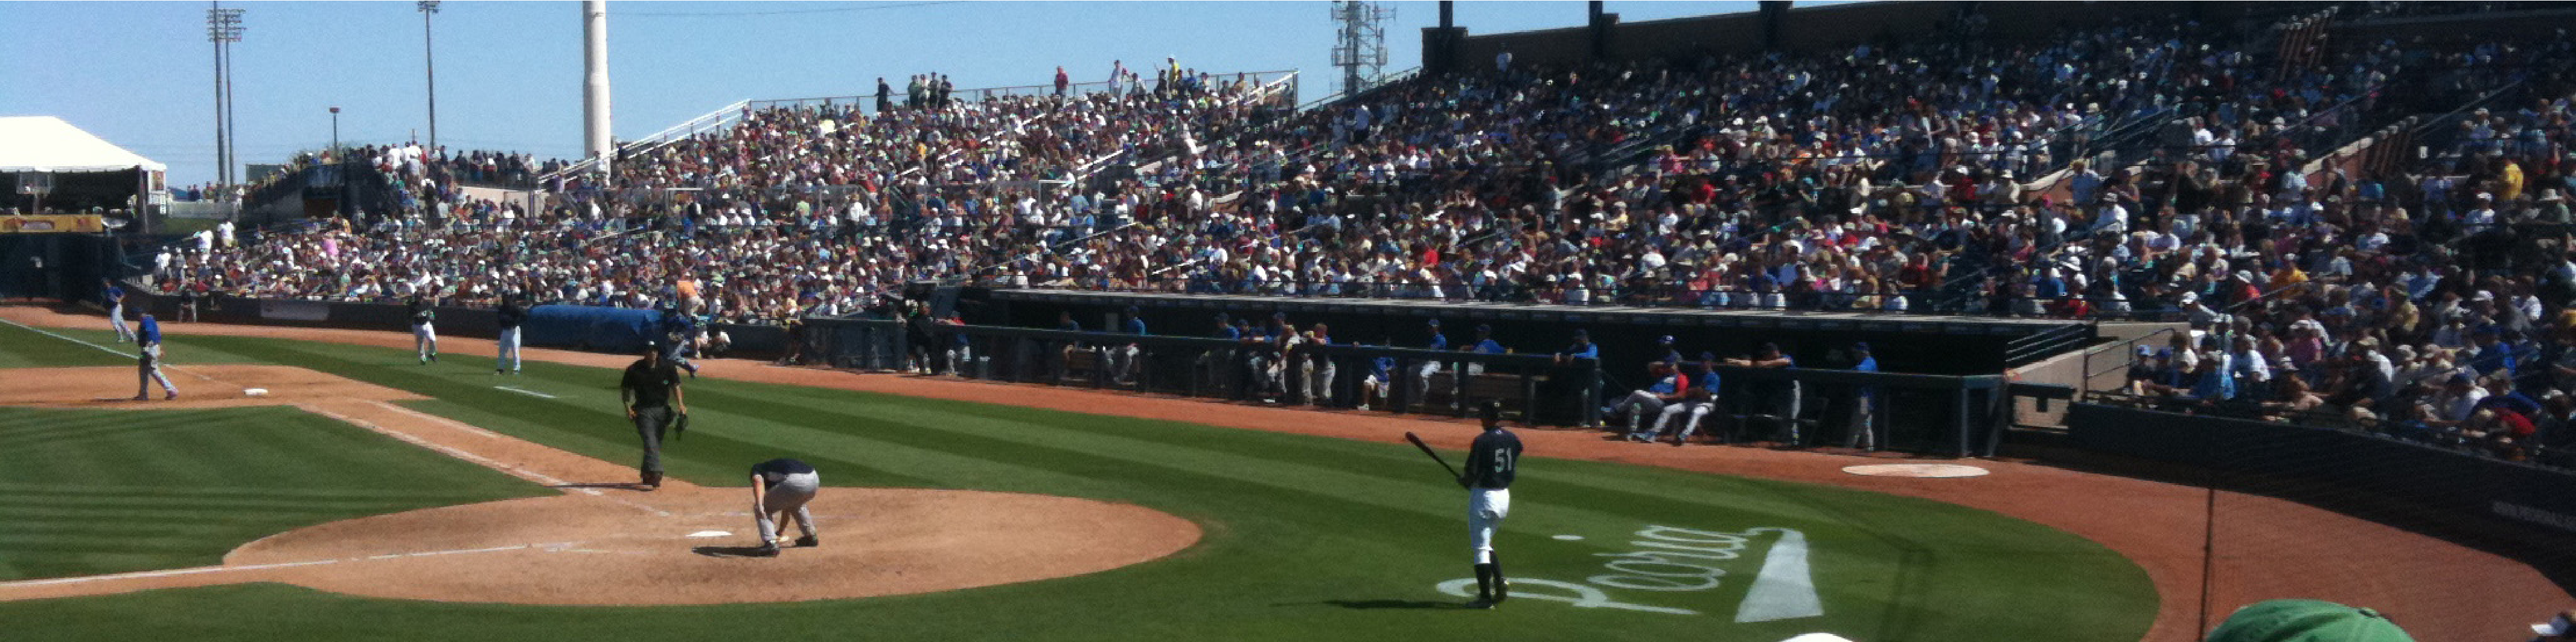
\includegraphics[height=1.5in]{images/sampleteaser}
%%   \caption{Spring Training 2009, Peoria, AZ.}
%% }

\maketitle

\begin{abstract}
We present a pipeline for translating user-specified 3D spline-based drawings to physical, 3D printed objects.  Our contributions are five-fold.  First, we present a graphical user interface in which users can easily draw B-Splines which can be fabricated.  Second, we provide an algorithm for generating a fabrication order of these splines which are consistent with support-based constraints, as well as a heuristic for ordering the splines and downsampling them to fabricable polylines.  Third, we provide inexpensive hardware specifications for providing a Kuka YouBot with a 3Doodler end-effector tool which interfaces with ROS.  Fourth, we provide a planning algorithm which enable the YouBots to plan collision-free paths with a working structure.  Finally, we provide an attempt at smooth velocity control which works for a variety of starting configurations and target trajectories, to mixed results.  We demonstrate our current results through simulation and by fabricating a few simple primitives.

TODO: Results

%Citations can be done this way~\cite{Jobs95} or this more concise  way~\shortcite{Jobs95}, depending upon the application.



\end{abstract}

%\begin{CRcatlist}
%  \CRcat{I.3.3}{Computer Graphics}{Three-Dimensional %Graphics and Realism}{Display Algorithms}
%  \CRcat{I.3.7}{Computer Graphics}{Three-Dimensional %Graphics and Realism}{Radiosity};
%\end{CRcatlist}

\keywordlist

%% Use this only if you're preparing a technical paper to be published in the 
%% ACM 'Transactions on Graphics' journal.

\TOGlinkslist

%% Required for all content. 

\copyrightspace

\section{Introduction}


%\begin{equation}
% \sum_{j=1}^{z} j = \frac{z(z+1)}{2}
%\end{equation}

%\begin{eqnarray}
%x & \ll & y_{1} + \cdots + y_{n} \\
%  & \leq & z
%\end{eqnarray}

TODO: talk about previous work, what we hope to do different and why we're the best, and goals.


\section{System Overview}
Our system pipeline consists of several interworking components, which we illustrate in figure \ref{fig:systemarchitecture}.  A general workflow is described as follows.  Users interact with our GUI in order to draw a set of splines, which represent the structure that they want the robot to draw.  When the user is satisfied with their drawing, she may choose to output it to a file readable to the robot fabrication.  In this output process, paths are ordered in a way that guarantees supports are generated before the splines which rest upon them while heuristically attempting to reduce potential for collisions.  In this process, the splines are also resized to a scale that fits a reasonably sized workspace for the robot, and approximated as a set of polylines, which make robot control easier.  The robot, a Kuka YouBot which is equipped with a 3Doodler on its end-effector, then reads in this file one polyline at a time.  For each polyline, it plans to achieve an initial configuration which is collision-free with the currently fabricated structure (which we call the working structure), and iteratively fabricates the polyline segment-wise using our robot control algorithm.  3Doodler interfacing is achieved through an Arduino control module, and we equip the robot with a spool of 2.85~mm PLA plastic so that the 3Doodler does not have to be re-filled.

\begin{figure}[t]{3.0in}
\centering
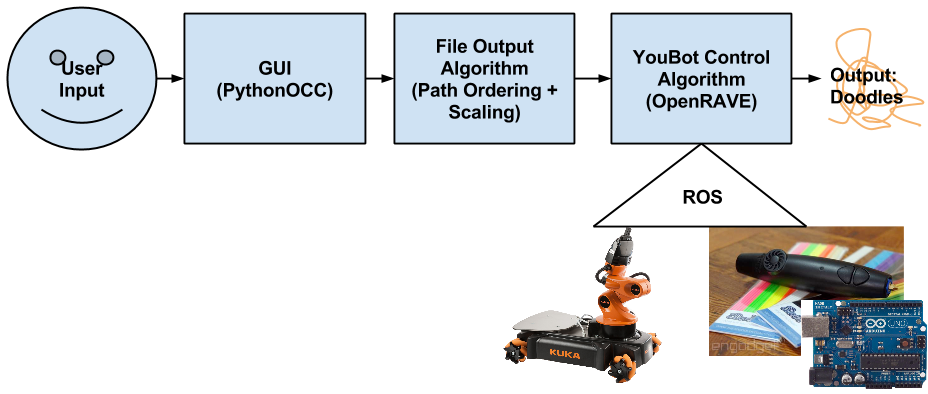
\includegraphics[width=3.0in]{images/system_arch.png}
\caption{A diagram of our 3Doodler pipeline.}
\label{fig:systemarchitecture}
\end{figure}

Our UI is built on top of PythonOCC \cite{PythonOCC}, an open source API for developing Computer-Aided Deisgn (CAD) software, which includes both visualization and geometric computing tools.  Our robotics infrastructure is built upon the Robot Operating System (ROS) \cite{ROS}.  OpenRAVE \cite{OpenRAVE} is used as a platform for computing inverse kinematics of the robot arm, as well as performing robot planning.




\section{Clamp Design}
Inspired by the idea of interchangeable tools for the YouBot \cite{Knepper13}, we developed a 3Doodler attachment which fits on the fingers of the YouBot as a glove.  The rings of the 3Doodler were tightly fitted to the form factor of the 3Doodler and away from its center where the 3Doodler is widest, so as to lock it firmly in place (TODO: it can still rotate though.  Address this). The clamp was 3D printed and coated in TangoBlack+ \cite{TangoBlack} to increase friction with the fingers and 3Doodler and decrease translational and rotational slip.  The design of a clamp half (a single finger) is shown in Fig. \ref{fig:halfclamp} and the printed version, complete with 3Doodler, can be found in Fig. \ref{fig:printedclamp}.  

\begin{figure}[t!]
\centering

\begin{subfigure}[t]{1.5in}
\centering
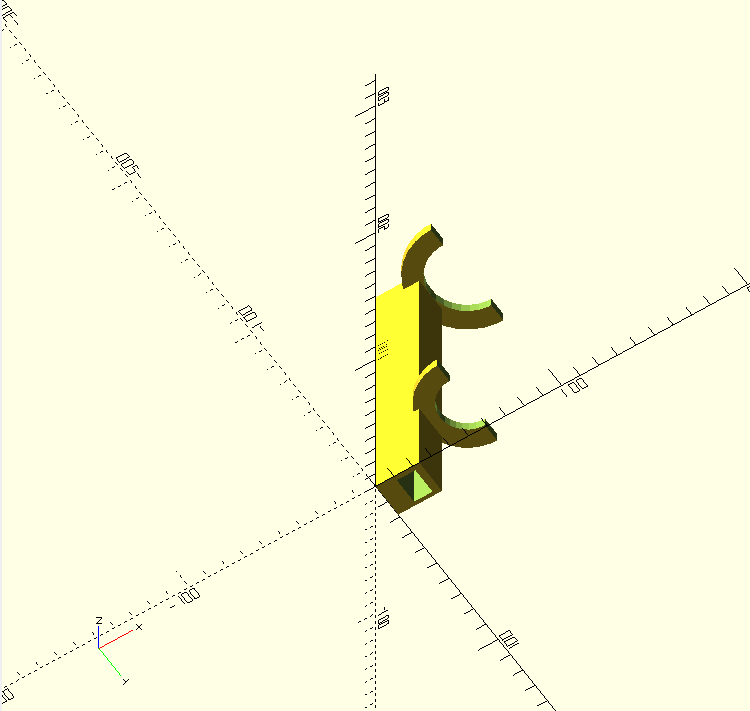
\includegraphics[width=1.5in]{images/clamp.png}
\caption{The OpenSCAD model of the Clamp for a single YouBot finger.}
\label{fig:halfclamp}
\end{subfigure}
~
\begin{subfigure}[t]{1.5in}
\centering
\includegraphics[width=1.5in]{images/clamp_printed.jpg}
\caption{The printed clamp with 3Doodler, affixed to the YouBot hand.}
\label{fig:printedclamp}
\end{subfigure}
\caption{The 3Doodler Clamp.}
\end{figure}



%TODO: talk about total load of YouBot and mass of clamp + doodler?

\section{Arduino Interface}
TODO: Vicki - describe interfacing, slow extrusion, fast extrusion, ROS interface, on/off sensing (if we have it), isReady detection, and a circuit diagram, if possible.


\section{UI Design}
TODO: Vicki
Note that we use cubic splines.

\section{Path Generation Algorithm}
In this section, we detail how our system converts our collection of B-Splines to ordered polylines for the YouBot to fabricate.  While the need to convert B-Splines into polylines is necessary for our algorithm, it may be tempting to simply order them for fabrication in the same order that they were drawn in the GUI.  This, however, is naïve for several reasons.  First, some splines may be unfabricable - splines which users draw suspended in mid-air, unattached to the ground or any other spline obviously cannot exist in the real world.  Further, consider Figure (TODO: make a good drawing).  Obviously, splines (TODO) cannot be fabricated before splines (TODO) which support them.  Further, for those splines which do not require support (e.g. those that lie on the ground), fabricating them outwardly will require no extra planning as the 3Doodler tool will never intersect with any of its pre-fabricated splines at any step.  However, fabricating them inwardly would require maneuvering the 3Doodler tool around the pre-fabricated splines to avoid collision.

In this section, we first explain how we transform a graph representing the splines and their connections into a tree in which any traversal, starting from the root, will never lead to fabricating a spline before its support.  Next, we describe a heuristic for traversing that tree in a way that hopes to simplify the collision-free motion planning problem.  Finally, we describe how we sample the splines and scale them to fit to a reasonable print volume.

\subsection{Constraint Generation}

Consider a graph $G = (V, E)$ where $V$ corresponds to the set of splines and there exists an edge $E$ between two nodes in $V$ when their corresponding splines are connected (for each connection).  With each edge $e_{ij} \in E$ connecting nodes $v_i$ and $v_j$ associate the minimum connection height of all points in which those two splines connect, $e_{ij}^z$
%$, and with each node $v_j \in V$, associate the height of %the minimum $e_i^z$ among all edges $e_i$ connected to %$v_j$ as $e_{min_z}$
.  Let $R \subseteq V$ be the root nodes of this graph, which correspond to splines which intersect the plane $z=0$.

TODO: clean up all this terminology to match algorithm.

Given this setup, we present an algorithm in Figure (TODO) for transforming this graph into a forest such that the fabrication of splines in any path from any root to a connected leaf guarantees that any spline's support will be built before it.  Note that as a limitation, this only considers geometric feasibility, and does not perform any sort of physical simulation to verify the stability of such a fabrication order.

\begin{algorithm}
\caption{Graph To Forest}\label{alg:graphtoforest}
\begin{algorithmic}[1]
\Procedure{GraphToForest}{}
\BState \textbf{Input:} $G$
\BState $pq \gets \textit{PriorityQueue()}$
\BState $F \gets \textit{Graph()}$ \Comment{We will build the output graph as $F$}.
\BState For each $r_i \in R$:
\State $F \gets F \cup \{r_i\}$
\State For each $e_{ij}$ connected to $r_i$
\State \hspace{\algorithmicindent} $pq.put( (r_i, e_{ij}), e_{ij}^z)$ \Comment{Put $(c_i, e_{ij}$ into the priority queue with priority $e_{ij}^z$.}

\BState While $pq \neq \emptyset$: \Comment{While the priority queue still has nodes}
\State $(v_i, e_{ij}^z) = pq.pop()$
\State if $v_j \notin F$:
\State \hspace{\algorithmicindent} $F \gets F \cup \{v_j, e_ij\}$
\State \hspace{\algorithmicindent} For each $e_{jk}$ connected to $v_j$
\State \hspace{\algorithmicindent} \hspace{\algorithmicindent} $pq.put( (v_j, e_{jk}), e_{jk}^z)$.
\BState \textbf{Output:} $F$

%\State $\textit{stringlen} \gets \text{length of %}\textit{string}$
%\State $i \gets \textit{patlen}$
%\BState \emph{top}:
%\If {$i > \textit{stringlen}$} \Return false
%\EndIf
%\State $j \gets \textit{patlen}$
%\BState \emph{loop}:
%\If {$\textit{string}(i) = \textit{path}(j)$}
%\State $j \gets j-1$.
%\State $i \gets i-1$.
%\State \textbf{goto} \emph{loop}.
%\State \textbf{close};
%\EndIf
%\State $i \gets i+\max(\textit{delta}_1(\textit{string}(i)),\textit{delta}_2(j))$.
%\State \textbf{goto} \emph{top}.
\EndProcedure
\end{algorithmic}
\end{algorithm}

We say a spline $a$ is supported by a spline $b$ if $b$'s lowest connection point is on $a$.

As an additional constraint, we require that for any two connected splines, they do not support each other.  This is something we eventually hope to be enforced by the GUI.

\begin{theorem}
Any traversal from a root to a connected leaf in the forest output by Algorithm \ref{alg:graphtoforest} will not lead to fabricating a spline before its support.
\end{theorem}



\begin{proof}
TODO: Is this good?
Proof by Induction.
Base case: We will always add a root node first, and since they intersect at $z=0$, they require no support.
Inductive case: Assume that through step $k$, no node has been added before its support.  Now, assume that at step $k+1$, we want to add a new spline $v_{k+1}$, that's connected to one of the existing splines in $F$.  We prove here that this must choose a spline that is supported by $F$.  Assume for contradiction's sake that $v_{k+1}$ is \emph{not} supported by the spline it is being attached to.  If that's the case, then it must be supported by a different spline $v'$ with a lower connect point which is not added yet.  But the only way that this spline could not be added yet is if it or some other spline on the path from the root  too $v'$ has a higher support point.  If this is the case though, it will have to be that either $v'$ and $v_{k+1}$ support each other or two splines on the path support each other (TODO: be more explicit here), which is not allowed.  Thus, we have a contradiction.


%any spline currently in $F$.  Then that must mean that it is supported by a spline that has not yet been added.  Call that spline $v'$.  But then, if $v'$ has not yet been added, its lowest connection point so far must be higher than that of $v_{k+1}$, because otherwise it would have been added.  

\end{proof}

Note that the way in which we "break cycles" here may not be unique, which may lead to suboptimal orderings in the subsequent step.


\subsection{Heuristic Ordering}
We wish to avoid moving the 3Doodler nozzle "inward," which could increase the difficulty of finding collision-free motion paths.  The resulting forest from the previous step provides the constraints on which order splines can be drawn (no spline on a tree can be drawn before its ancestor) but we are otherwise free to traverse the forest in any order that we wish, starting from the set of root nodes.  Here, we provide a heuristic for doing so in a way that reduces the odds of moving significantly "inward" in our drawing.  Define a point $a$ and being more inner than $b$ if $a$ is closer than $b$ to the centroid axis-aligned bounding box (AABB) of our spline set.  Observe that the only way we could move our 3Doodler nozzle monotonically outward is if we order our splines by increasing distance to the centroid of their innermost point (although, also note that such an ordering does not \emph{guarantee} that we can move monotonically outward as such an ordering typically does not exist; the intuition however is that such a phenomenon may roughly occur several times as we move upward in $z$).

In other words, define the heurstic function of a spline $h(v) = -d(c, \min_t(v(t))$, where $c$ is the centroid of the drawing's AABB and $v(t)$ is the value of spline $v$ at parameter point $t$.  We perform a depth-first traversal of our forest, choosing the lowest heuristic function as it's available.  This generates our path ordering.

TODO: Should I put an algorithm?


\subsection{Polyline Conversion}
Since fabricating continuous splines is difficult, we simplify the problem by approximating splines as polylines.  This process is comprised of three steps.

The first step is, for each polyline in our ordering, we choose a threshold value $V$ (which will correspond to the resolution of our polyline, i.e. the length of each segment) and calculate a threshold $T$ which satisfies $\forall t_{max} > t > t' > 0, |t' - t| < T \rightarrow ||v(t') - v(t)||_2 < V$ (PythonOCC provides functionality for calculating this value).  We then sample $v$ at increments of $T$. to create a list of candidate points $C$ for our polyline.  

Next, we scale and center our points in $C$ (analogous to a normalizing procedure, but uniformly among all dimensions) in order to fit the drawing within a predetermined print volume.  In practice, we set the $x$ and $y$ ranges to 10~cm, the $z$ range to 4~cm, and centered the output drawing at $(0, 0, 0)$.

For each point in $C$ we then greedily add to an output list $C'$ the next point when its distance from the previously added point is at least $V$ (PythonOCC does not provide functionality for arclength, and rather than attempt to write code to approximate it, we assume that for splines with sufficiently small curvature and small $V$ that using this distance should not destroy much information about the polyline).  We also add to $C'$ the closest point to each connection point, which should be helpful for making sure the material is at the connection point (we should add the connection point itself but it's not yet clear to us how to determine where in $C'$ it should be inserted).  In practice, we keep $V$ relatively small, at 1~cm.

\section{YouBot Control}

In this section we detail the algorithm used for controlling the algorithm and extruding material.  We note that \emph{arm control} and \emph{base control} are used exclusively; the arm and base are never moving simultaneously.  This simplifies our problem by avoiding the difficulty of having to synchronize arm and base movement.  Further, arm motions are used exclusively for drawing line segments of the polylines, while base movements are used to move the YouBot in order to prepare for the next segment.

\subsection{Arm Control}

\subsection{Base Control}

\section{YouBot Planning and Collision Avoidance}

\section{Results}

\section{Conclusion}

\subsection{Future Work}



\section*{Acknowledgements}

Mehmet Dogar and Robert Katzschmann, for suggestions for fixing the YouBot arm control when it wasn't working, which still didn't work.



\bibliographystyle{acmsiggraph}
\bibliography{template}





\end{document}
